\documentclass{article}
\usepackage{graphicx}
\usepackage{geometry}
\geometry{margin=1in}

\title{Report on Faast-A-Faas-Framework}
\author{Arijit Saha (210050017) and Aryan Mathe (210050021)}
\date{}

\begin{document}
\maketitle

\section{Introduction}
Faast-A-Faas-Framework is a project designed to evaluate and compare different
cluster configurations for Function as a Service (FaaS) platforms. The goal is
to analyze performance metrics such as latency, throughput, and resource
utilization across various setups. This report provides an overview of the
project's approach, including the types of clusters tested, the workloads used
for evaluation, and instructions for setting up and running experiments. By
offering insights into the impact of different configurations, this project
aims to guide best practices for optimizing serverless infrastructure

\section{Cluster Configurations}
The project considers the following cluster configurations:

\subsection{Single Pod Cluster}
\nobreak
\begin{figure}
    \begin{minipage}[u]{0.6\textwidth}
        %\flushleft
        This configuration consists of a single pod with a single container deployed on
        a single-node cluster. The pod hosts the FaaS service, and all incoming
        requests are directed to the single container within the pod. This simple setup
        serves as a baseline for comparison with other configurations.
    \end{minipage}%
    \hfill
    \begin{minipage}[u]{0.4\textwidth}
        \centering
        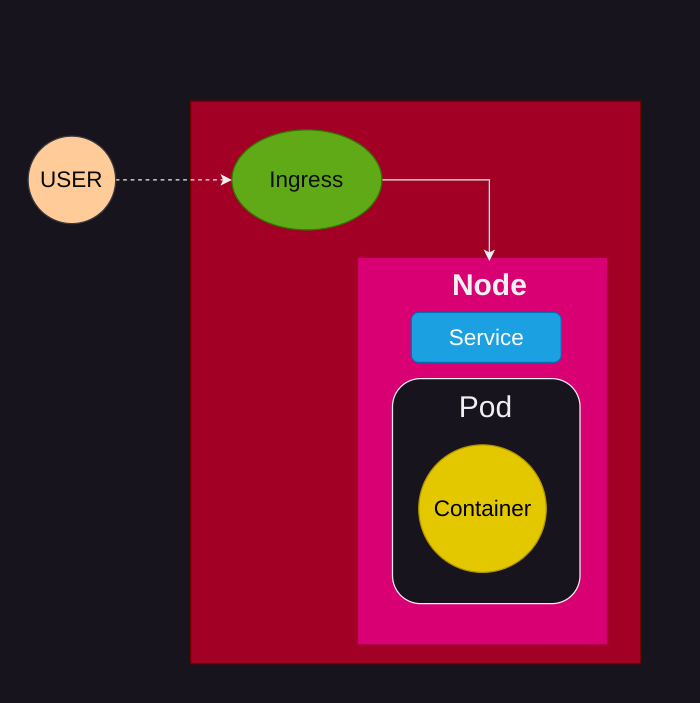
\includegraphics[width=0.4\textwidth]{../images/single_pod.png}
        \caption{Single Pod Cluster}
        \label{fig:single_pod_cluster}
    \end{minipage}
\end{figure}


\subsection{Single Pod with Multi-Container}
\nobreak
\begin{figure}[h]
    \begin{minipage}[b]{0.6\textwidth}
        \flushleft
        In this configuration, a single pod contains multiple containers that run the
        FaaS service on a single-node cluster. An Nginx load balancer pod is also
        deployed to route incoming requests to the containers within the pod. This
        setup allows testing the efficiency of using multiple containers within a
        single pod.
    \end{minipage}%
    \hfill
    \begin{minipage}[b]{0.4\textwidth}
        \centering
        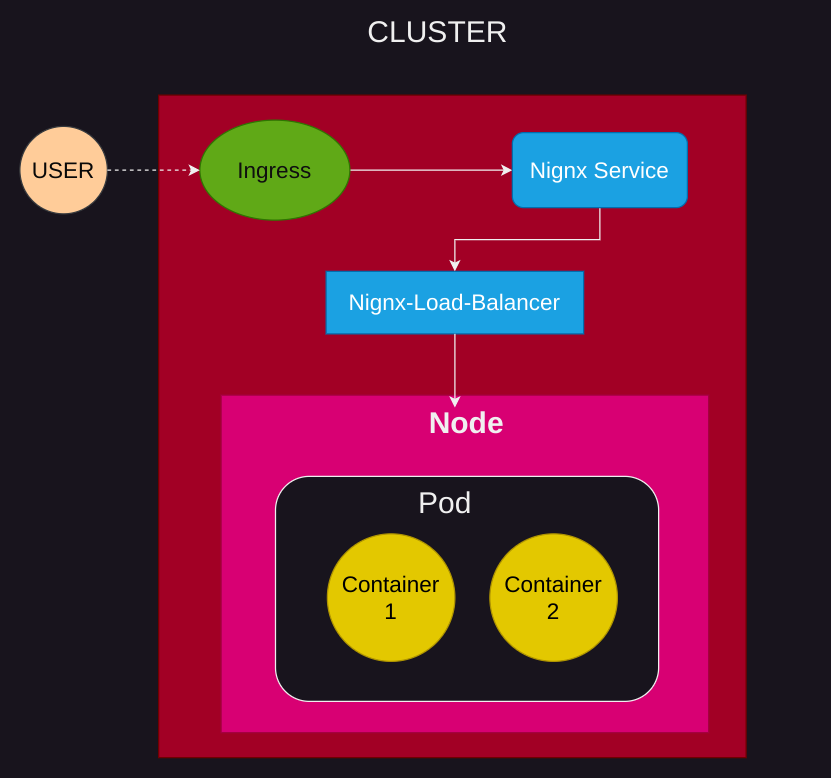
\includegraphics[width=0.4\textwidth]{../images/one_pod_two_container.png}
        \caption{Single Pod with Multi-Container}
        \label{fig:single_pod_multi_container}
    \end{minipage}
\end{figure}


\subsection{Multi-Pod with Single Node}
\nobreak
\begin{figure}[h]
    \begin{minipage}[b]{0.6\textwidth}
        \flushleft
        This configuration includes multiple pods, each with one container running the
        FaaS service, deployed on a single node. An Nginx load balancer pod manages
        incoming requests, routing them to the appropriate FaaS service pods. This
        setup tests how multiple pods interact within a single node and the impact of
        load balancing.
    \end{minipage}%
    \hfill
    \begin{minipage}[b]{0.4\textwidth}
        \centering
        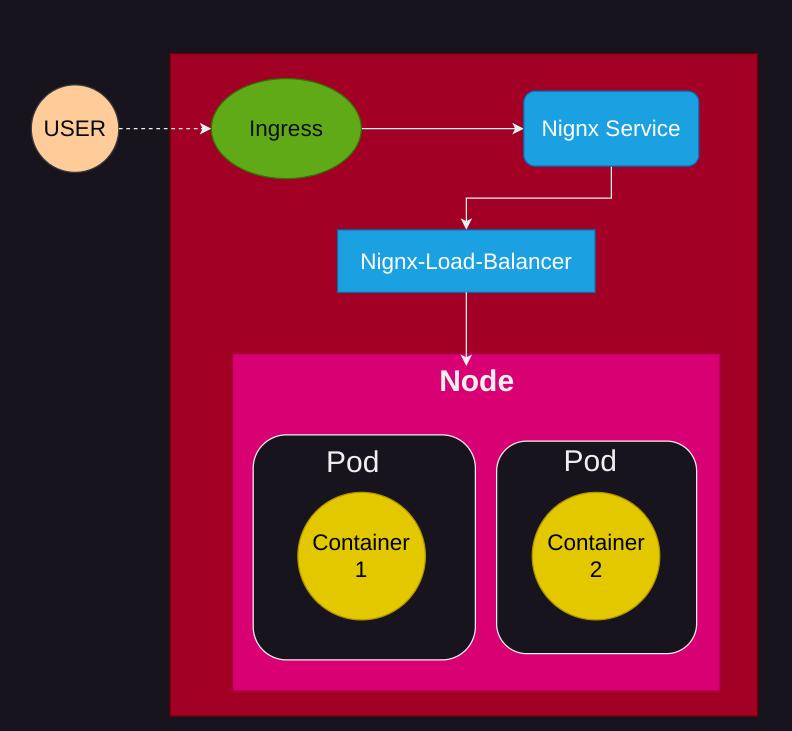
\includegraphics[width=0.4\textwidth]{../images/one_node_two_pod.png}
        \caption{Multi-Pod with Single Node}
        \label{fig:multi_pod_single_node}
    \end{minipage}
\end{figure}



\subsection{Multi-Pod with Multi-Node}
\nobreak
\begin{figure}[h]
    \begin{minipage}[b]{0.6\textwidth}
        \flushleft
        In this configuration, multiple pods are distributed across two different
        nodes, with each pod containing one container running the FaaS service. An
        Nginx load balancer pod manages incoming requests, distributing them evenly
        across the different nodes and their pods. This setup tests how the system
        performs when multiple pods are deployed across multiple nodes.
    \end{minipage}%
    \hfill
    \begin{minipage}[b]{0.4\textwidth}
        \centering
        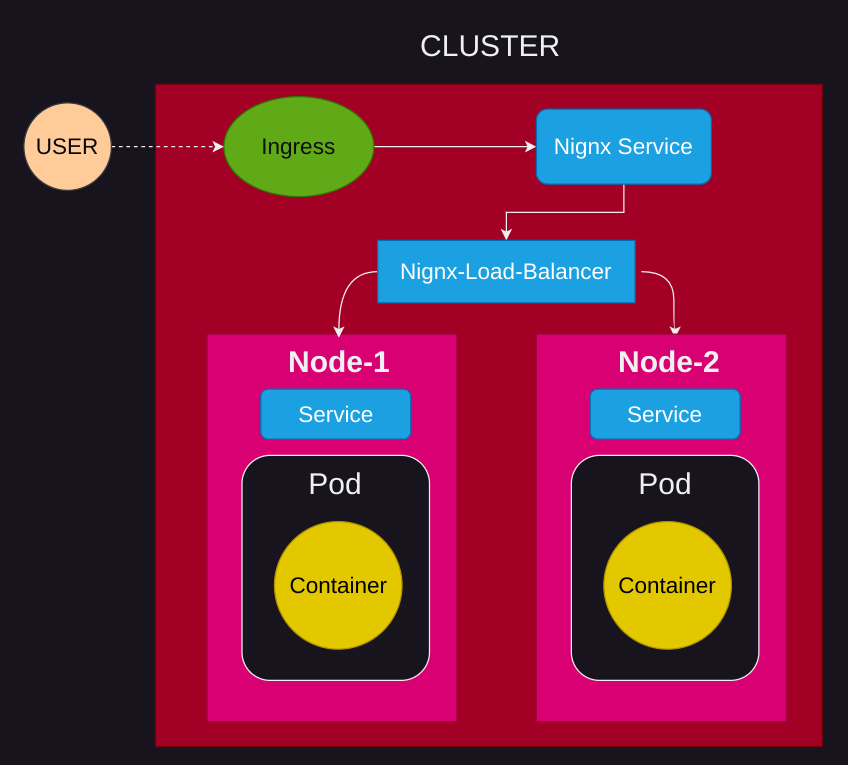
\includegraphics[width=0.4\textwidth]{../images/two_node.png}
        \caption{Multi-Pod with Multi-Node}
        \label{fig:multi_pod_multi_node}
    \end{minipage}
\end{figure}


\subsection{Horizontal Pod Autoscaler (HPA)}
\nobreak
\begin{figure}[h]
    \begin{minipage}[b]{0.6\textwidth}
        \flushleft
        The Horizontal Pod Autoscaler (HPA) is a Kubernetes feature that automatically
        scales the number of pods in response to changes in resource utilization or
        other metrics. In this configuration, multiple pods (initially one) are
        deployed on a single node. The HPA monitors resource usage (such as CPU or
        memory) and dynamically adjusts the number of pods based on predefined
        thresholds, ensuring efficient resource usage and consistent performance.
    \end{minipage}%
    \hfill
    \begin{minipage}[b]{0.4\textwidth}
        \centering
        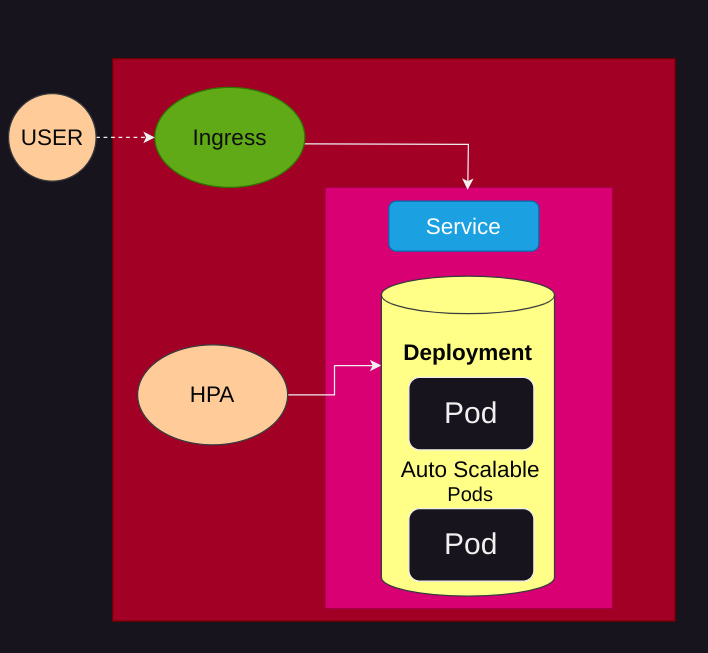
\includegraphics[width=0.4\textwidth]{../images/hpa.png}
        \caption{Horizontal Pod Autoscaler}
        \label{fig:hpa}
    \end{minipage}
\end{figure}

\subsection{Vertical Pod Autoscaler (VPA)}
\begin{figure}[h]
    \begin{minipage}[b]{0.6\textwidth}
        \flushleft
        The Vertical Pod Autoscaler (VPA) is a Kubernetes feature that adjusts the
        resource limits and requests of a pod based on its actual usage. In this
        configuration, a single pod is deployed with VPA enabled in a single-node
        cluster. The VPA monitors the pod's resource usage and dynamically adjusts its
        resource requests and limits to ensure optimal performance and resource
        efficiency.
    \end{minipage}%
    \hfill
    \begin{minipage}[b]{0.4\textwidth}
        \centering
        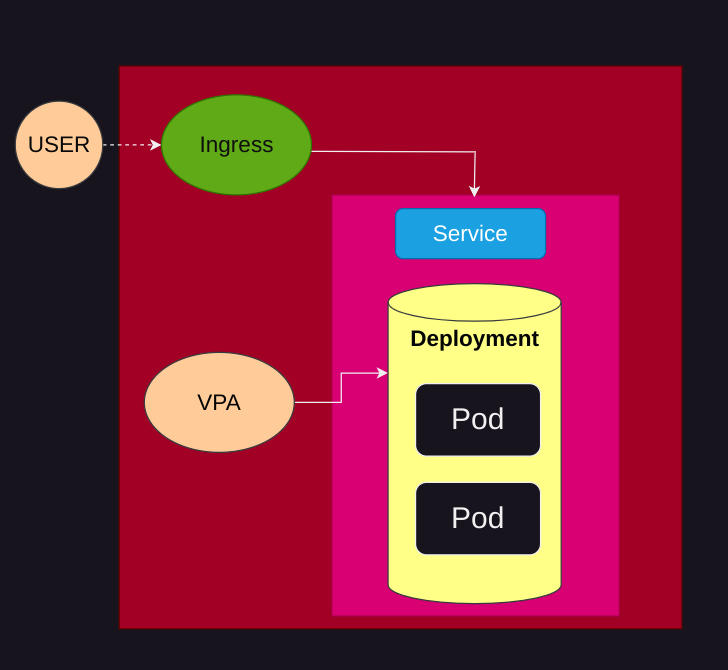
\includegraphics[width=0.4\textwidth]{../images/vpa.png}
        \caption{Vertical Pod Autoscaler}
        \label{fig:vpa}
    \end{minipage}
\end{figure}
\newpage
\section{Metrics}
This section discusses the metrics used to evaluate the performance and resource utilization of the Function as a Service (FaaS) platform across different cluster configurations. The two main types of workloads tested were a simple loop and a large Lorem Ipsum generator.

\subsection{Latency and Throughput}
Latency and throughput are critical performance metrics for evaluating FaaS services:

\begin{itemize}
    \item \textbf{Latency:} The time taken for a request to be processed by the FaaS service and return a response. Lower latency is generally preferred as it indicates faster response times and better user experience.
    \item \textbf{Throughput:} The number of requests that can be processed per unit of time. Higher throughput signifies the ability to handle more requests concurrently and efficiently.
\end{itemize}

To measure these metrics, the `wrk` tool was used to simulate load on the FaaS service and capture response times and request rates. `wrk` was configured to send a defined number of requests to the service for each cluster configuration. The results were then analyzed to determine the average latency and throughput.

\subsection{Resource Utilization (CPU and Memory)}
Resource utilization is another important aspect of evaluating FaaS services:

\begin{itemize}
    \item \textbf{CPU Usage:} The amount of CPU resources consumed by the FaaS service. Lower CPU usage is preferred as it indicates efficient use of processing power.
    \item \textbf{Memory Usage:} The amount of memory consumed by the FaaS service. Lower memory usage is desirable as it implies efficient use of available memory resources.
\end{itemize}

Resource usage was measured using the Kubernetes `metrics-server` API, which provides real-time data on the CPU and memory usage of pods and containers within the cluster. This data was collected and analyzed for each cluster configuration.

\subsection{Workloads for Testing}
The project tested the FaaS platform using two types of simple workloads:

\begin{itemize}
    \item \textbf{Beautiful Loops:} This workload runs a for loop performing simple computations, providing insight into the performance of the FaaS service under repetitive tasks.
    \item \textbf{Large Lorem Ipsum Generator:} This workload generates a large block of Lorem Ipsum text and returns it as a response, testing the service's ability to handle data-heavy tasks and manage memory usage efficiently.
\end{itemize}

These workloads were chosen to provide a diverse set of scenarios for testing the FaaS service. The results of latency, throughput, and resource utilization were measured and compared across different cluster configurations.

In summary, these metrics help assess the FaaS platform's performance and resource usage under varying conditions, providing valuable insights for optimizing serverless applications.

\section{Workloads for Testing}
The project uses two types of simple stateless workloads to test various cluster environments:

\subsection{Beautiful Loops}
This workload runs a for loop performing some simple computations.

\subsection{Random Weird Text}
This workload generates some random text and returns it as a response.

\section{Requirements}
To run the experiments, the following tools need to be installed:

\begin{itemize}
   \item docker
   \item kubectl
   \item minikube
   \item helm
\end{itemize}

\section{Running Instructions for Setting up a Cluster Environment}
To set up the environment for running cluster configurations, run the following command:

\begin{verbatim}
bash setup.sh
\end{verbatim}

The supported app-types based on the cluster configurations defined above are:

\begin{verbatim}
single-pod  two-pod-same-node  two-pod-diff-node  hpa  vpa  two-container
\end{verbatim}

%To set up the requirements for running clusters, run the following command with the appropriate `<app_type>`:

\begin{verbatim}
bash deploy_app.sh <app_name> <app_type> <docker_image_name> <python-app-file> <requirements-file> <port> <map_url>
\end{verbatim}

\section{Generating Analysis Results}
To generate analysis results, follow these steps:

\begin{enumerate}
   \item Set up the `metrics-server` REST-API by running the following command in two different terminal windows:
   
   \begin{verbatim}
   minikube dashboard --port=20000
   \end{verbatim}
   
   \item Run the following command to perform the analysis for different cluster configurations and generate logs for response-time and resource utilization:
   
   \begin{verbatim}
   bash src/analysis/perform_analysis.sh <host> <url> <app-type> <app-name>
   \end{verbatim}
   
   This will generate logs for response-time and resource utilization based on the defined workload. The file names will be in the following format:
   
   \begin{verbatim}
   <logs-dir>/<app-name>-<app-type>-response_time.csv
   <logs-dir>/<app-name>-<app-type>-resource_usage.csv
   \end{verbatim}
   
   \item Execute the following Python file to generate plots for the analysis:
   
   \begin{verbatim}
   python3 analysis/get_plot_from_log.py
   usage: script to generate plot from log files [-h] --app-type APP_TYPE
                                                 [--response-log RESPONSE_LOG]
                                                 [--resources-log RESOURCES_LOG] --output-folder
                                                 OUTPUT_FOLDER --app-name APP_NAME

   options:
     -h, --help            show this help message and exit
     --app-type APP_TYPE   single-pod/two-pod-same-node/two-pod-diff-node/hpa/vpa/two-container
     --response-log RESPONSE_LOG
     --resources-log RESOURCES_LOG
     --output-folder OUTPUT_FOLDER
     --app-name APP_NAME
   \end{verbatim}
\end{enumerate}

\end{document}
